\section{Umsetzung des realen Clusters}
\label{sec:realCluster}

\begin{wrapfigure}{r}{0.4\columnwidth}
    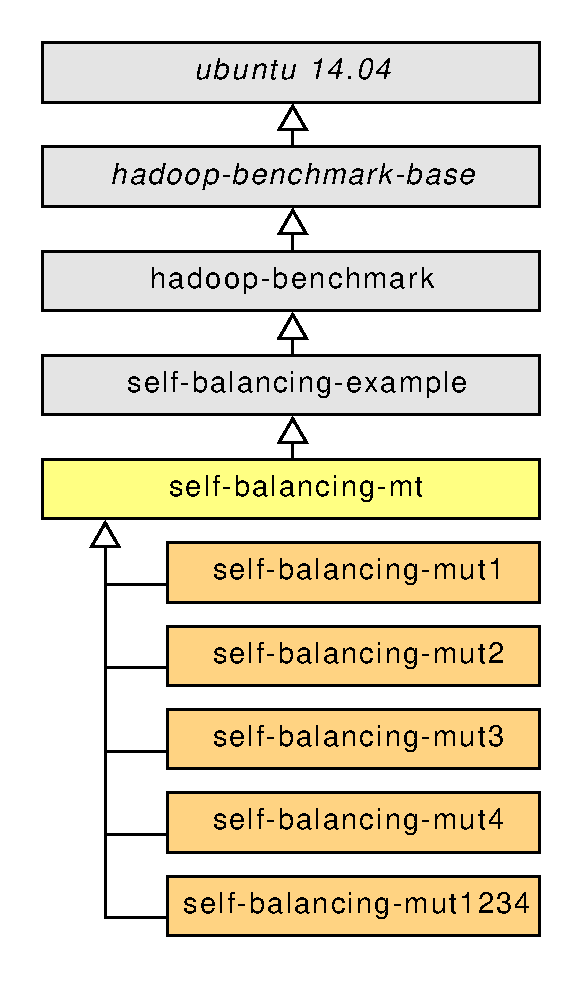
\includegraphics[width=0.4\columnwidth]
    {./resources/hadoopBenchDockerInherits.pdf}
    \caption[Vererbungshierarchie der Docker"=Images in Hadoop"=Benchmark]
    {Vererbungshierarchie der Docker"=Images in Hadoop"=Benchmark.
    Die kursiv markierten Images können nicht mithilfe von Hadoop"=Benchmark gestartet werden, die grau unterlegten Images sind bereits in Hadoop"=Benchmark enthalten bzw. benötigt.}
    \label{fig:hadoopBenchDockerInherits}
\end{wrapfigure}

Das reale Cluster wurde mithilfe der Plattform Hadoop"=Benchmark umgesetzt.
Hierzu wurden speziell für diese Fallstudie verschiedene Szenarien entwickelt, mithilfe denen das Cluster mit den benötigten Einstellungen bzw. den zu testenden Mutanten gestartet wurde.
Um die Verwaltung des Clusters zu vereinfachen wurden zudem entsprechende Setup- und Startscripte entwickelt, die auch von den implementierten Connectoren genutzt wurden.

\subsection{Grundlegender Aufbau}
\label{subsec:clusterBasics}

Da Docker (genutzt wird hier Version 18.03 CE) und Hadoop vor allem zum Einsatz in Linux"=Umgebungen entwickelt wurden, werden für das reale Cluster bis zu zwei physische Linux"=Hosts genutzt.
Auf einem dieser beiden Hosts wird mithilfe von VirtualBox 5.2 eine VM mit Windows 10 Education Version 1803 ausgeführt, um die Tests mithilfe von \gls{ss} auszuführen.
Dies ist nötig, da \gls{ss} mithilfe des .NET"=Frameworks entwickelt wurde (vgl. \cref{sec:ssharp}), welches auf Linux in Form von .NET Core zudem nur in einem verringertem Funktionsumfang verfügbar ist \cite{Schwichtenberg2017}.

Die beiden Hosts sind jeweils mit einem Intel Core i5"=4570 @ 3,2 GHz x 4, 16 GB Arbeitsspeicher sowie einer SSD ausgestattet, auf der Ubuntu 16.04 LTS als Betriebssystem installiert ist.

Insgesamt wurden für diese Fallstudie die 6 in \cref{fig:hadoopBenchDockerInherits} gelb bzw. orange hinterlegten Szenarien mit den entsprechenden Docker"=Images entwickelt.
Das zentrale Image in dieser Fallstudie ist das gelb hinterlegte \texttt{self-balancing-mt}, in dem alle benötigten angepassten Einstellungen enthalten sind.
Dies betrifft \zB die Anpassung der Zeitabstände zur Erkennung von defekten Nodes oder das Starten des \gls{TLS}, welcher in den Standard"=Szenarien der Plattform nicht gestartet wird.
Die orange hinterlegten Images dienen zur Ausführung der  Mutationstests.
Die Images enthalten daher nur die mutierte Selfbalancing"=Komponente, welche dadurch die in \texttt{self-balancing-example} enthaltene überschreiben.
Das Namenssuffix der Images bzw. Szenarien in Form der Nummern geben an, welche der in \cref{sec:implMutationTests} generierten Mutationen enthalten sind.

\subsection{HostMode des Clusters}
\label{subsec:hostMode}

Der bereits mehrfach erwähnte \texttt{HostMode} beschreibt den prinzipiellen Aufbau des gestarteten Clusters.
Es ist hierbei möglich, das Cluster wie in \cref{sec:hadoopBenchmark} beschrieben mithilfe von Docker Machine zu starten, wodurch entsprechende VMs gestartet werden, auf denen das Cluster auf Docker"=Containern ausgeführt wird.
Der größte Nachteil dieses \texttt{DockerMachine}"=Modes ist, dass das Cluster nicht bzw. nur umständlich auf mehreren Hosts ausgeführt werden kann.

Um das Cluster auf beiden für diese Fallstudie genutzten Hosts auszuführen, wurde daher der \texttt{Multihost}"=Mode entwickelt, bei dem die Docker"=Container des Clusters direkt auf den jeweiligen Hosts ohne Docker Machine gestartet werden:

\begin{figure}[h]
    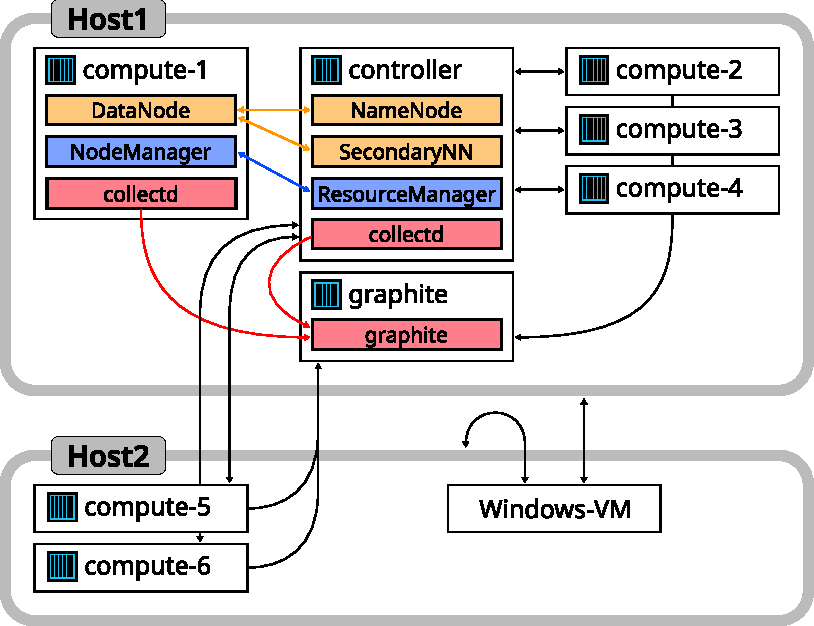
\includegraphics{./resources/caseStudyHadoopSetup.pdf}
    \caption[Cluster"=Setup bei der Nutzung des Multihost"=Modes]
    {Cluster"=Setup bei der Nutzung des \texttt{Multihost}"=Modes.
    Hier ist das konkrete, in dieser Fallstudie genutzte Setup gezeigt.
    Grün: HDFS, Blau: YARN, Rot: Graphite.}
    \label{fig:caseStudyHadoopSetup}
\end{figure}

Die genaue Anzahl der zu nutzenden Hosts und der Hadoop"=Nodes ist in beiden \texttt{HostMode}s variabel, wodurch es auch möglich ist, das Cluster nur auf Host1 zu starten.
Damit das Cluster jedoch auf beiden Hosts gestartet werden kann, ist es nötig, zuvor beide Hosts als Docker"=Swarm miteinander zu verbinden.
Außerdem können mithilfe des \texttt{Multihost}"=Modes dem Hadoop"=Cluster weitere, sonst für die Ausführung der VMs benötigte Ressourcen, zur Verfügung gestellt werden, weshalb in dieser Fallstudie der \texttt{Multihost}"=Mode genutzt wurde.
Beim \texttt{Mutihost}"=Mode werden zudem nur auf Host1 die volle Anzahl an definierten Nodes pro Host gestartet, auf allen anderen Hosts wird jeweils die Hälfte gestartet und ausgeführt.

Je nach \texttt{HostMode} unterscheiden sich einzelne Pfade oder Adressen, \zB die der REST"=API.
Auch aus diesem Grund wurde die bereits in \cref{subsec:modelClass} erläuterte Klasse \texttt{ModelSettings} entwickelt, welche die Verwaltung der entsprechenden Pfade und Adressen übernimmt.

\subsection{Setup- und Startscripte}
\label{subsec:scripts}

Die Plattform Hadoop"=Benchmark enthält bereits zum Starten des Clusters ein Setup"=Script und zum Ausführen der Benchmarks entsprechende Start"=Scripte (vgl. \cref{sec:hadoopBenchmark}).
Um die Interaktion aufgrund der beiden unterschiedlichen \texttt{HostMode}s zu vereinfachen, wurde für jeden \texttt{HostMode} ein Setup"=Script entwickelt, um eine einheitliche und vereinfachte Befehlssyntax bereitzustellen.
Die beiden entwickelten Setup"=Scripte werden vom \texttt{CmdConnector} genutzt um die benötigten Aktionen auf dem Cluster auszuführen (vgl. \cref{subsubsec:implCmdConnector}).
Die beiden Setup"=Scripte abstrahieren somit die vom \texttt{HostMode} abhängigen, benötigten Befehle und sorgen dafür, dass der genutzte \texttt{HostMode} transparent ist, benötigen hierfür jedoch die gleiche, in \cref{app:setupScriptCmds} gezeigte, Befehlssyntax.
Sie beinhalten entsprechende Befehle für folgende Aktionen:

\begin{itemize}
    \item Starten und Beenden des gesamten Clusters
    \item Injizieren und Reparieren von Komponentenfehlern
    \item Ausführen von \gls{CLI}"=Befehlen von Hadoop
\end{itemize}

Zudem wird beim Starten des Clusters immer geprüft, ob sich die Dockerfiles geändert haben und entsprechend die Docker"=Images aktualisiert, aus denen das Cluster gestartet wird.
Die Setup"=Scripte enthalten außerdem weitere, jeweils spezifische Befehle zum Umgang mit dem Cluster im entsprechenden \texttt{HostMode}.

Zum zentralen Starten der Benchmarks wurde ebenfalls ein zentrales Benchmark"=Startscript entwickelt, welches die jeweiligen Start"=Scripte der einzelnen Benchmarks ausführt.
Dadurch kann analog zum Setup"=Script unabhängig vom zu startenden Benchmark vom \texttt{CmdConnector} immer der gleiche Syntax genutzt werden.
Das zentrale Benchmark"=Startscript ermittelt basierend auf dem zu startenden Benchmark das jeweils benötigte Start"=Script und übergibt die jeweils benötigten Parameter.
Die vom \texttt{HostMode} abhängigen Parameter zum Starten der Benchmark"=Container werden von den hierfür angepassten Start"=Scripten der Benchmarks selbst ermittelt.
Die jeweiligen Startparameter der Anwendungen selbst werden vom Benchmark"=Controller (vgl. \cref{subsec:appImplementation}) bereitgestellt.
